\documentclass[../main.tex]{subfiles}
\graphicspath{{\subfix{../images/}}}
\begin{document}

\begin{figure}[h!]
    \centering
    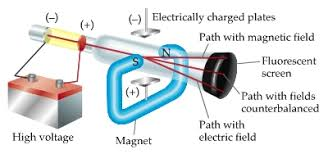
\includegraphics[scale=0.9]{images/08.JJ-Thomson..jpg}
    \caption{Autre schéma réaliste}
    \label{fig:my_label}
\end{figure}

\begin{enumerate}
    \item On voit, dans le dispositif ci-dessus, un générateur branché à une cathode et à une anode.
    \item Les électrons passent ensuite dans le tube et continuent jusqu'aux deux plaques métalliques.
    \item Celle du dessus est chargée négativement et celle du dessous est chargée positivement.
    \item Il y a un aimant en forme de O coupé au milieu pour le tube, qui se situe à l'extérieur du tube donc.
    \item La trajectoire des électrons va monter en présence d'un champ magnétique, va descendre en présence d'un champ électrique et  va aller tout droit quand les champs sont contre-balancés. 
    \item 
\end{enumerate}
\end{document}